\documentclass[10pt]{article}
\usepackage[cm]{fullpage}
\usepackage{amsmath,amssymb}
\usepackage{hyperref}
\usepackage{algorithm,algorithmic}
\usepackage{graphicx}
\newcommand{\Uspace}{\mathbb{U}}
\newcommand{\Vspace}{\mathbb{V}}
\newcommand{\Wspace}{\mathbb{W}}
\newcommand{\Hdiv}{\texttt{HDiv}}
\newcommand{\Hcurl}{\texttt{HCurl}}
\renewcommand{\vec}[1]{\boldsymbol{#1}}
\newcommand{\zhat}{\hat{\vec{z}}}
\newcommand{\ddt}[1]{\frac{\partial #1}{\partial t}}
\newcommand{\ddtdisc}[1]{\frac{{#1}^{(t+\Delta t)}-{#1}^{(t)}}{\Delta t}}
\newcommand{\tavg}[1]{\frac{{#1}^{(t+\Delta t)}+{#1}^{(t)}}{2}}
\title{Matrix-free 3d solver for linear gravity wave test case}
\date{\today}
\author{Eike Hermann M\"{u}ller, Department of Mathematical Sciences, University of Bath}
\begin{document}
\maketitle
%%%%%%%%%%%%%%%%%%%%%%%%%%%%%%%%%%%%%%%%%%%%%%%
\section{Problem formulation}
%%%%%%%%%%%%%%%%%%%%%%%%%%%%%%%%%%%%%%%%%%%%%%%
%%%%%%%%%%%%%%%%%%%%%%%%%%%%%%%%%%%%%%%%%%%%%%%
\subsection{Continuous equations}
%%%%%%%%%%%%%%%%%%%%%%%%%%%%%%%%%%%%%%%%%%%%%%%
Consider the following linear gravity wave problem \cite{McRae2014} for the pressure $p$, velocity $\vec{u}$ and buoyancy $b$:
\begin{xalignat}{3}
   \ddt{\vec{u}} &= \nabla p + b \zhat, &
   \ddt{p} &= -c^2 \nabla\cdot \vec{u}, &
   \ddt{b} &= -N^2\vec{u}\cdot\zhat.
\label{eqn:ContinuousEquations}
\end{xalignat}
For simplicity we assume that both the speed of sound $c$ and the buoyancy frequency $N$ are constant and enforce the boundary condition
\begin{equation}
 \vec{u}\cdot\vec{n}=0\label{eqn:BoundaryCondition}
\end{equation}
at the upper and lower boundary of the atmosphere.
%%%%%%%%%%%%%%%%%%%%%%%%%%%%%%%%%%%%%%%%%%%%%%%
\subsection{Finite element discretisation}
%%%%%%%%%%%%%%%%%%%%%%%%%%%%%%%%%%%%%%%%%%%%%%%
%%%%%%%%%%%%%%%%%%%%%%%%%%%%%%%%%%%%%%%%%%%%%%%
\paragraph{Function spaces.}
%%%%%%%%%%%%%%%%%%%%%%%%%%%%%%%%%%%%%%%%%%%%%%%
We have the following de Rham complexes in one, two and three dimensions:
\begin{xalignat}{3}
  \Vspace_0 \overset{\partial_z}{\rightarrow}\Vspace_1,&
  &\Uspace_0 \overset{\nabla^{\perp}}{\rightarrow}
\Uspace_1 \overset{\nabla\cdot}{\rightarrow}\Uspace_2, &
  &\Wspace_0 \overset{\nabla}{\rightarrow} \Wspace_1 \overset{\nabla\times}{\rightarrow} \Wspace_2\overset{\nabla\cdot}{\rightarrow} \Wspace_3
\end{xalignat}
with
\begin{equation}
 \begin{aligned}
  \Wspace_0 &= \Uspace_0\otimes\Vspace_0,\\
  \Wspace_1 &= \Hcurl(\Uspace_1\otimes\Vspace_0)\oplus
\Hcurl(\Uspace_0\otimes\Vspace_1),\\
  \Wspace_2 &= \Hdiv(\Uspace_2\otimes\Vspace_0)\oplus
\Hdiv(\Uspace_1\otimes\Vspace_1),\\
  \Wspace_3 &= \Uspace_2\otimes\Uspace_1.
 \end{aligned}
\end{equation}
$\Wspace_2^0$ denotes the space of all functions in $\Wspace_2$ which satisfy the boundary condition (\ref{eqn:BoundaryCondition}). We write $\Wspace_2^v \equiv \Hdiv(\Uspace_2\otimes\Vspace_0)$ and $\Wspace_2^v\equiv\Hdiv(\Uspace_1\otimes\Vspace_1)$ for the vertical and horizontal components of the velocity space, and the buoyancy lives in the space $\Wspace_2^b\equiv \Uspace_2\otimes\Vspace_0$. Note that $\Wspace_2^v=\Hdiv(\Wspace_2^b)$, so the function spaces have the same number of degrees of freedom but differ in how they are pulled back to the reference element. Then the fields in (\ref{eqn:ContinuousEquations}) live in the following spaces:
\begin{xalignat}{3}
  \vec{u} &\in \Wspace_2^0=\Wspace_2^{v,0}\oplus\Wspace_2^{h,0},&
  b &\in \Wspace_2^b, &
  p &\in \Wspace_3.
\end{xalignat}
For ease of notation, we will not make the boundary condition on $\vec{u}$ explicit in the following, and will write $\Wspace_2$ where it should really be $\Wspace_2^0$ etc.
The lowest order function spaces are illustrated in Fig. \ref{fig:functionspaces}.
\begin{figure}
 \begin{center}
  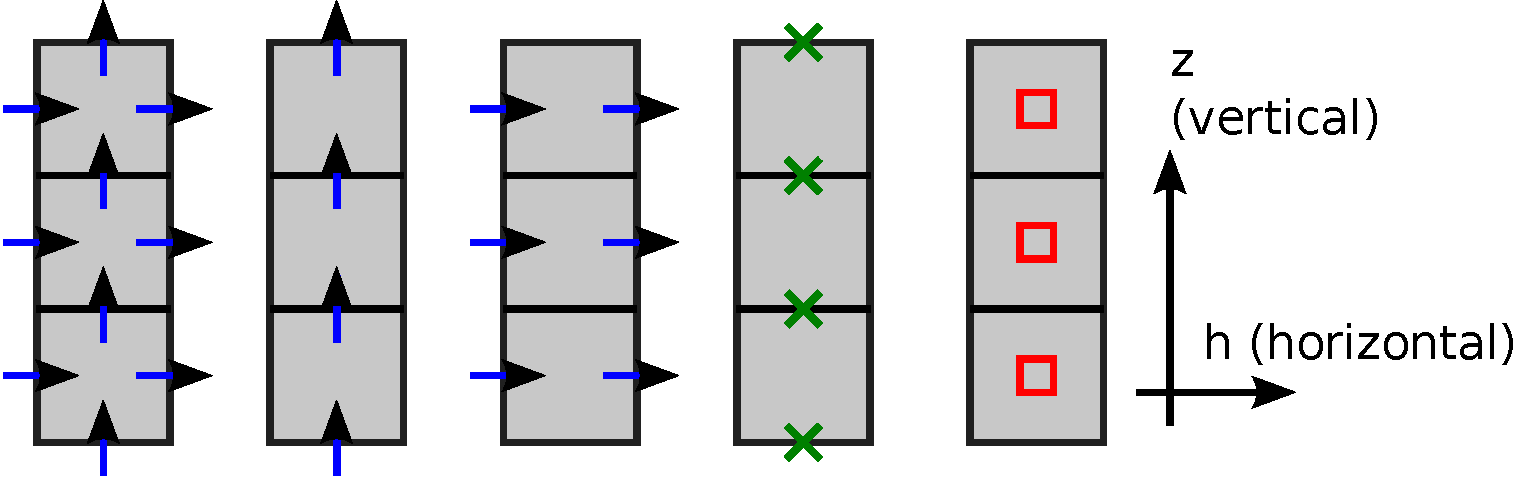
\includegraphics[width=0.6\linewidth]{functionspaces.pdf}
 \end{center}
 \caption{Function spaces at lowest order from left to right: $\Wspace_2$ (velocity), $\Wspace_2^v = \Hdiv(\Uspace_2\otimes\Vspace_0)$ (vertical component of velocity), $\Wspace_2^h=\Hdiv(\Uspace_1\otimes\Vspace_1)$ (horizontal/tangential component of velocity), $\Wspace_2^v=\Uspace_2\otimes\Vspace_0$ (buoyancy), $\Wspace_3$ (pressure).}
\label{fig:functionspaces}
\end{figure}
%%%%%%%%%%%%%%%%%%%%%%%%%%%%%%%%%%%%%%%%%%%%%%%
\paragraph{Discrete equations.}
%%%%%%%%%%%%%%%%%%%%%%%%%%%%%%%%%%%%%%%%%%%%%%%
Multiply with test functions $\vec{w}\in \Wspace_2$, $\phi\in \Wspace_3$ and $\gamma\in\Wspace_2^b$ and use the implicit midpoint rule to discretise in time:
\begin{equation}
 \begin{aligned}
  &\langle\vec{w},\ddtdisc{\vec{u}}\rangle
  - \langle\nabla\cdot\vec{w},\tavg{p}\rangle
  - \langle\vec{w},\tavg{b}\zhat\rangle = 0\\[1ex]
  &\langle\phi,\ddtdisc{p}\rangle
  +c^2 \langle\phi,\nabla\cdot\tavg{\vec{u}}\rangle
  = 0\\[1ex]
  &\langle\gamma,\ddtdisc{b}\rangle
  + N^2\langle\gamma,\tavg{\vec{u}}\cdot\zhat\rangle
  = 0
 \end{aligned}
\end{equation}
Define $\delta p\equiv p^{(t+\Delta t)}-p^{(t)}$, $p_0\equiv p^{(t)}$ etc. and note that $\tavg{p}=\frac{\delta p}{2}+p_0$ to obtain a system of equations for the increments $\delta\vec{u}$, $\delta p$ and $\delta b$
\begin{equation}
 \begin{aligned}
  &\langle\vec{w},\delta\vec{u}\rangle
  - \frac{\Delta t}{2}\langle\nabla\cdot\vec{w},\delta p\rangle
  - \frac{\Delta t}{2}\langle\vec{w},\delta b\zhat\rangle
  = \Delta t \langle\nabla\cdot\vec{w},p_0\rangle
  + \Delta t \langle\vec{w},b_0\zhat\rangle
  \equiv r_u
 \\[1ex]
  &\langle\phi,\delta p\rangle
  +\frac{\Delta t}{2}c^2\langle\phi,\nabla\cdot\delta\vec{u}\rangle
  = -\Delta tc^2\langle\phi,\nabla\cdot\vec{u}_0\rangle
  \equiv r_\phi
  \\[1ex]
  &\langle\gamma,\delta b\rangle
  + \frac{\Delta t }{2}N^2\langle\gamma,\delta\vec{u}\cdot\zhat\rangle
  = -\Delta t N^2\langle\gamma,\vec{u}_0\cdot\zhat\rangle
  \equiv r_b\label{eqn:Increments}
 \end{aligned}
\end{equation}
%%%%%%%%%%%%%%%%%%%%%%%%%%%%%%%%%%%%%%%%%%%%%%%
\paragraph{Matrix formulation.}
%%%%%%%%%%%%%%%%%%%%%%%%%%%%%%%%%%%%%%%%%%%%%%%
By introducing the mass matrices
\begin{xalignat}{3}
  M_u:\Wspace_2\rightarrow\Wspace_2,\left(M_u\right)_{ij} &\equiv \langle \vec{w}_i\cdot\vec{w}_j\rangle,&
  M_p:\Wspace_3\rightarrow\Wspace_3,\left(M_p\right)_{ij} &\equiv \langle \phi_i,\phi_j\rangle, &
  M_b:\Wspace_2^b\rightarrow\Wspace_2^b,\left(M_b\right)_{ij} &\equiv \langle \gamma_i,\gamma_j \rangle
\end{xalignat}
and the derivative- and projection operators
\begin{xalignat}{2}
  D:\Wspace_2\rightarrow \Wspace_3,\left(D\right)_{ij} &\equiv \langle\phi_i,\nabla\cdot\vec{w}_j\rangle, &
  Q:\Wspace_2^b\rightarrow \Wspace_2,\left(Q\right)_{ij} &\equiv \langle\vec{w}_i,\gamma_j\zhat\rangle,
\end{xalignat}
the system of equations (\ref{eqn:Increments}) can be written as a matrix equation for the dof-vectors $\vec{U}$ (velocity), $\vec{P}$ (pressure) and $\vec{B}$ (buoyancy):
\begin{equation}
\begin{pmatrix}
  M_u & 
    -\frac{\Delta t}{2}D^T & 
    -\frac{\Delta t}{2}Q\\[1ex]
  \frac{\Delta t}{2}c^2D & M_p & 0\\[1ex]
  \frac{\Delta t}{2}N^2Q^T & 0 & M_b
\end{pmatrix}
\begin{pmatrix}
  \vec{U}\\[1ex]\vec{P}\\[1ex]\vec{B}
\end{pmatrix}
=
\begin{pmatrix}
  M_u\vec{R}_u\\[1ex]M_p\vec{R}_p\\[1ex]M_b\vec{R}_b
\end{pmatrix}.\label{eqn:MixedSystem}
\end{equation}
Use the third equation to eliminate the buoyancy  \footnote{In the absence of orography this equation is satisfied pointwise, i.e. $\vec{B}=\vec{R}_b-\frac{\Delta t}{2}N^2\vec{U}$.}
\begin{equation}
\vec{B}=\vec{R}_b-\frac{\Delta t}{2}N^2M_b^{-1} Q^T\vec{U}
\label{eqn:BuoyancyBacksubstitution}
\end{equation}
and insert it into the velocity equation to obtain a mixed system for pressure and velocity:
\begin{equation}
  A\begin{pmatrix}\vec{P}\\[1ex]\vec{U}\end{pmatrix}
  \equiv
  \begin{pmatrix}
   M_p & \frac{\Delta t}{2}c^2 D \\[1ex]
   -\frac{\Delta t}{2}D^T & \tilde{M}_u
  \end{pmatrix}
  \begin{pmatrix}\vec{P}\\[1ex]\vec{U}\end{pmatrix}
 =
\begin{pmatrix}M_p\vec{R}_p\\[1ex]M_u\tilde{\vec{R}}_u\end{pmatrix}
\qquad\text{with}\quad 
\tilde{M}_u \equiv M_u + \omega^2_N QM_b^{-1}Q^T
\quad\text{and}\quad \omega_N \equiv \frac{\Delta t}{2}N\label{eqn:PressureVelocitySystem}
\end{equation}
We also have for the new RHS
\begin{equation}
  \tilde{\vec{R}}_u = \vec{R}_u+\frac{\Delta t}{2}M_u^{-1}Q\vec{R}_b.
  \label{eqn:BuoyancyRHS}
\end{equation}
In the absence of orography, $Q=Q^T=M_b$. In any case, both $M_b$ and $\tilde{M}_u$ (and $M_u$) are well conditioned, so can be inverted with a small number of (unpreconditioned) Richardson- or CG- iterations.
%%%%%%%%%%%%%%%%%%%%%%%%%%%%%%%%%%%%%%%%%%%%%%%
\section{Schur complement Preconditioner}
%%%%%%%%%%%%%%%%%%%%%%%%%%%%%%%%%%%%%%%%%%%%%%%
The inverse of the operator $A$ in (\ref{eqn:PressureVelocitySystem}) is given by
\begin{equation}
  A^{-1} = 
\begin{pmatrix}
  1 & 0 \\[1ex]
  \frac{\Delta t}{2}\tilde{M}_u^{-1} D^T & 1
\end{pmatrix}
\begin{pmatrix}
  H^{-1} & 0 \\[1ex] 0 & \tilde{M}_u^{-1}
\end{pmatrix}
\begin{pmatrix}
  1 & -\frac{\Delta t}{2}D\tilde{M}_u^{-1} \\[1ex]
  0 & 1
\end{pmatrix}\label{eqn:SchurComplement}
\end{equation}
with the (positive-definite) ``Helmholtz'' operator
\begin{equation}
  H \equiv M_p + \omega_c^2 D\tilde{M}_u^{-1} D^T
\qquad\text{where}\quad \omega_c \equiv \frac{\Delta t}{2}c.
  \label{eqn:HelmholtzOperator}
\end{equation}
Explicitly, the preconditioner for the full mixed system in (\ref{eqn:MixedSystem}) can be written as in Algorithm \ref{alg:mixed_preconditioner}:
\begin{algorithm}[H]
 \caption{Preconditioner for mixed system (\ref{eqn:MixedSystem}); given $M_u\vec{R}_u$, $M_p\vec{R}_p$ and $M_b\vec{R}_b$ calculate $\vec{U}$, $\vec{P}$ and $\vec{B}$.}
 \label{alg:mixed_preconditioner}
 \begin{algorithmic}[1]
   \STATE{Calculate $(M_u\tilde{\vec{R}}_u)=(M_u\vec{R}_u)-\frac{\Delta t}{2}QM_b^{-1}(M_b\vec{R}_b)$} \COMMENT{Modified right hand side for velocity}
   \STATE{Calculate $(M_p\tilde{\vec{R}}_p)=(M_p\vec{R}_p)-\frac{\Delta t}{2}D\tilde{M}_u^{-1}(M_u\tilde{\vec{R}}_u)$} \COMMENT{Modified right hand side for pressure}
  \STATE{Solve $H\vec{P}=(M_p\tilde{\vec{R}}_p)$ for $\vec{P}$} \COMMENT{Pressure solve}
  \STATE{Calculate $\vec{U}=\tilde{M}_u^{-1}\left((M_u\tilde{\vec{R}}_u)+\frac{\Delta t}{2}D^T \vec{P}\right)$} \COMMENT{Velocity backstubstitution}
  \STATE{Calculate $\vec{B}=M_b^{-1}\left((M_b\vec{R}_b)-\frac{\Delta t}{2}N^2 Q^T \vec{U}\right)$} \COMMENT{Buoyancy backstubstitution}
 \end{algorithmic}
\end{algorithm}
To (approximately) invert $H$, we can use another suitably preconditioned CG iteration.
We precondition $H$ with a similar operator $\hat{H}$ in which we neglect the couplings between $\Wspace_2^v=\Hdiv(\Uspace_2\otimes\Vspace_0)$ and $\Wspace_2^v=\Hdiv(\Uspace_1\otimes\Vspace_1)$ [step (i)], set $Q=Q_T=M_b$ [step (ii)]  and approximate the inverses of the mass matrices in $\Wspace_2^v=\Hdiv(\Uspace_2\otimes\Vspace_0)$ and $\Wspace_2^h=\Hdiv(\Uspace_1\otimes\Vspace_1)$ by lumped mass matrices [step (iii)].
The first two approximations are exact in the absence of orography.
More explicitly, this series of approximations can be written down as follows:
\begin{equation}
 \begin{aligned}
  D\tilde{M}_u^{-1}D^T&=
\left(D_h,D_z\right)
\begin{pmatrix}
  \tilde{M}_{u,h} & \tilde{M}_{u,hz}\\
  \tilde{M}_{u,hz}^{T} & \tilde{M}_{u,z}
\end{pmatrix}^{-1}
\begin{pmatrix}
  D_h^T\\D_z^T
\end{pmatrix}\\[1ex]
&\overset{\text{step (i)}}{\approx}
\left(D_h,D_z\right)
\begin{pmatrix}
  \tilde{M}_{u,h} & 0\\
  0 & \tilde{M}_{u,z}
\end{pmatrix}^{-1}
\begin{pmatrix}
  D_h^T\\D_z^T
\end{pmatrix}
=
D_h\left(\tilde{M}_{u,h}\right)^{-1}D_h^T + 
D_z \left(\tilde{M}_{u,z}\right)^{-1}D_z^T\\[1ex]
&\overset{\text{step (ii)}}{\approx}
D_h\left(M_{u,h}\right)^{-1}D_h^T + 
\frac{1}{1+\omega_N^2}D_z \left(M_{u,z}\right)^{-1}D_z^T\\[1ex]
&\overset{\text{step (iii)}}{\approx}
D_h M_{u,h,\text{inv}}D_h^T + 
\frac{1}{1+\omega_N^2}D_z M_{u,z,\text{inv}}D_z^T
\end{aligned}
\end{equation}
In the first step we could also have used a better approximation of $\tilde{M}_u^{-1}$ by using the Schur-complement of the velocity mass matrix.
We defined the mass matrices in the horizontal and vertical velocity spaces as
\begin{xalignat}{2}
M_{u,h}:\Wspace_2^h\rightarrow\Wspace_2^h,\left(M_{u,h}\right)_{ij} &\equiv \langle \vec{w}^{(h)}_i\cdot\vec{w}^{(h)}_j\rangle,&
M_{u,z}:\Wspace_2^z\rightarrow\Wspace_2^z,\left(M_{u,z}\right)_{ij} &\equiv \langle \vec{w}^{(z)}_i\cdot\vec{w}^{(z)}_j\rangle
\end{xalignat}
and the derivative operators as 
\begin{xalignat}{2}
D_h:\Wspace_2^h\rightarrow \Wspace_3,\left(D_h\right)_{ij} &\equiv \langle\phi_i,\nabla\cdot\vec{w}^{(h)}_j\rangle, &
D_z:\Wspace_2^z\rightarrow \Wspace_3,\left(D_z\right)_{ij} &\equiv \langle\phi_i,\nabla\cdot\vec{w}^{(z)}_j\rangle.
\end{xalignat}
The basis functions of these spaces are listed in Tab. \ref{tab:basisfunctions}.
\begin{table}
 \begin{center}
  \begin{tabular}{|l|rr|rr|rrr|}
    \hline
    Function space & 
      $\Uspace_1$ & $\Uspace_2$ & 
      $\Vspace_0$ & $\Vspace_1$ &
      $\Wspace_3$ & $\Wspace_2^v$ & $\Wspace_2^h$\\
    \hline
    basis function &
      $\tau_i(\vec{x})$ & $\sigma_i(\vec{x})$ &
      $\alpha_k(\vec{x})$ & $\beta_k(\vec{x})$ &
      $\phi_i=\left(\sigma(\vec{x})\beta(\vec{x})\right)_i$ &
        $\vec{w}_i^{(z)}=\Hdiv\left(\sigma(\vec{x})\alpha(\vec{x})\right)_i$ &
        $\vec{w}_i^{(h)}=\Hdiv\left(\tau(\vec{x})\beta(\vec{x})\right)_i$\\
    \hline
  \end{tabular}
 \end{center}
 \caption{Basis functions}
 \label{tab:basisfunctions}
\end{table}

$M_{u,h,\text{inv}}$ and $M_{u,z,\text{inv}}$ are approximations to $M_{u,h}^{-1}$ and $M_{u,z}^{-1}$. In the simplest case $M_{u,h,\text{inv}}$ could be the diagonal matrix defined as
\begin{equation}
  \left(M_{u,h,\text{inv}}\right)_{ij} \equiv \delta_{ij}/\left(M_{u,h}\right)_{ii}\qquad\text{for all $i$}. 
\label{eqn:horizontalMassLumping}
\end{equation}
$M_{u,z}$ does not contain any couplings in the horizontal direction, i.e. the global matrix is block diagonal (with each block corresponding to couplings between dofs in one column). In each of the blocks we can, for example, construct a sparse approximate inverse \cite{Grote1997} of the local banded matrix to obtain $M_{u,z,\text{inv}}$.

In summary we have for the approximate Helmholtz operator:
\begin{equation}
  \hat{H} = M_{p} + \omega_c^2\left(
  D_h M_{u,h,\text{inv}} D_h^T +
\frac{1}{1+\omega_N^2}D_z M_{u,z,\text{inv}} D_z^T\right)
\label{eqn:Preconditioner}
\end{equation}

Since $\Uspace_2$ is a DG space, there will be no couplings between different columns for $M_p$, $M_{u,z}$, $M_{u,z,\text{inv}}$ and $D_z$, in other words the global matrices are block-diagonal (with each block corresponding to the couplings in one vertical column). Similarly, since $\Vspace_1$ is a DG space, there are no couplings between the dofs in different vertical layers in $M_{p}$, $M_{u,h}$ and $M_{u,h,\text{inv}}$, but this is not relevant here.

In the smoother we need the block-diagonal $\hat{H}_z$ of (\ref{eqn:Preconditioner}), i.e. in each column we need to construct the banded matrix which would be obtained from $\hat{H}$ is we neglected all couplings between neighbouring columns (but keep the strong couplings in the vertical direction). In each column we can obtain the entries of this matrix as
\begin{equation}
  \Delta_h:\Wspace_3 \rightarrow\Wspace_3,\quad \Delta_h \equiv \text{diag}_{h}\left(D_h M_{u,h,\text{inv}} D_h^T\right)
\end{equation}
with
\begin{equation}
  \left(\Delta_h\right)_{ij}
  = \sum_{k,\ell} 
\left(D_h\right)_{ik} 
\left(M_{u,h,\text{inv}}\right)_{k\ell}
\left(D^T_h\right)_{\ell j}.\label{eqn:Deltah}
\end{equation}
Here $i$ and $j$ are restricted to the indices of the $\Wspace_3$ dofs in the same column.

In summary, the block-diagonal (denoted by $\text{diag}_h(\cdot)$) of the Helmholtz operator is given as
\begin{equation}
  \text{diag}_h(\hat{H}) = \hat{H}_z \equiv M_{p} + \omega_c^2\Delta_h+\frac{\omega_c^2}{1+\omega_N^2} D_z M_{u,z,\text{inv}} D_z^T
  \label{eqn:HHgeneralbanded}.
\end{equation}
In each vertical column the matrix representations of all operators in (\ref{eqn:HHgeneralbanded}), i.e. $M_p$, $\Delta_h$, $D_z$ and $M_{u,z,\text{inv}}$, can be written as generalised banded matrices which will be discussed in section \ref{sec:BandedMatrices}.
%%%%%%%%%%%%%%%%%%%%%%%%%%%%%%%%%%%%%%%%%%%%%%%
\section{Implementation}
%%%%%%%%%%%%%%%%%%%%%%%%%%%%%%%%%%%%%%%%%%%%%%%
%%%%%%%%%%%%%%%%%%%%%%%%%%%%%%%%%%%%%%%%%%%%%%%
\subsection{Algorithmic components}
%%%%%%%%%%%%%%%%%%%%%%%%%%%%%%%%%%%%%%%%%%%%%%%
The system in (\ref{eqn:MixedSystem}) can be solved with a preconditioned Krylov space iteration (e.g. GMRES or BiCGStab). For this we need to be able to carry out the following operations:
\begin{itemize}
  \item Apply the operator on the left hand side of (\ref{eqn:MixedSystem}). This can be done either in a matrix-free way or by using the LMA representation of the operators $M_b$, $M_p$, $M_u$, $D$ and $Q$.
  \item Calculate the modified RHS in (\ref{eqn:BuoyancyRHS}) and back-substitute the buoyancy according to (\ref{eqn:BuoyancyBacksubstitution}). In addition to operator applications, this requires solving for the buoyancy mass matrix $M_b$, which can be achieved with an (unpreconditioned) CG iteration since the matrix $M_b$ is well conditioned.
  \item Invert the triangular matrices on a vector $(\vec{P},\vec{U})$ and calculate the lower right block in (\ref{eqn:SchurComplement}), i.e. calculate $\tilde{M}_u^{-1}\vec{U}$. In addition to operator applications as above, this will require solves for the modified mass matrix $\tilde{M}_u$, which can again be achieved by a (unpreconditioned) CG iteration. Applying the operator $\tilde{M}_u$ in this iteration requires inverting $M_b$, but again this is possible (see above).
  \item (Approximately) invert the operator $H$ in (\ref{eqn:HelmholtzOperator}). For this, use a Krylov iteration (e.g. CG) with $H$ and precondition it with the operator $\hat{H}$ in (\ref{eqn:Preconditioner}). For this we need to be able to
  \begin{itemize}
    \item Apply the operator $H$ in (\ref{eqn:HelmholtzOperator}). This is possible if we can apply $D$ and (approximately) invert $\tilde{M}_u$, as described above.
    \item Approximately invert $\hat{H}$ to precondition $H$. For this we use a multigrid iteration. The most important ingredient is the smoother application $p\mapsto p+\hat{H}_z^{-1}(r_p-\hat{H}p)$ and it requires us to
    \begin{itemize}
      \item Construct suitable lumped operators $M_{u,h,\text{inv}}$ and $M_{u,z,\text{inv}}$.
      \item Apply the operator $\hat{H}$ in (\ref{eqn:Preconditioner}). For this we need to be able to apply the additional operators $M_p$, $D_h$, $D_z$, $M_{u,h,\text{inv}}$ and $M_{u,z,\text{inv}}$. Note that these require the new function spaces $\Wspace_2^h$ and $\Wspace_2^v$, so we need to be able to assemble operators mapping to these spaces.
      \item Construct and invert the block-diagonal operator $\hat{H}_z$ by doing banded matrix solves in each column. This is discussed in section \ref{sec:BandedMatrices}.
    \end{itemize}
  \end{itemize}
\end{itemize}

It is worth stressing that, since they are only required in the preconditioner, any mass matrix solves for $M_b$, $M_u$ and $\tilde{M}_u$ above can be (i) carried with a small number of CG or Richardson iterations or (ii) be approximated by inverting suitably lumped matrices. In addition, bear in mind that in general (but not here, since we are only looking at the linearised equations) the linear operator is used inside a Newton iteration, and hence further simplications might be possible without compromising the convergence of the outer Newton loop.
%%%%%%%%%%%%%%%%%%%%%%%%%%%%%%%%%%%%%%%%%%%%%%%
\subsection{Generalised banded matrices}\label{sec:BandedMatrices}
%%%%%%%%%%%%%%%%%%%%%%%%%%%%%%%%%%%%%%%%%%%%%%%
As described above, in each column all components of the operator in (\ref{eqn:HHgeneralbanded}) can be represented by (generalised) banded matrices. In the following we describe this data structure and its algebra.

Consider an $n_A\times m_A$ banded matrix $A$ (representing an operator mapping from $\mathbb{R}^{m_A} \rightarrow \mathbb{R}^{n_A}$) which only has entries for indices $(i,j)$ which satisfy
\begin{equation}
  -\gamma_-^{(A)} \le \alpha^{(A)}i-\beta^{(A)}j \le \gamma_+^{(A)}.
\end{equation}
An example is shown in Fig. \ref{fig:bandedmatrix}.
\begin{figure}
 \begin{center}
  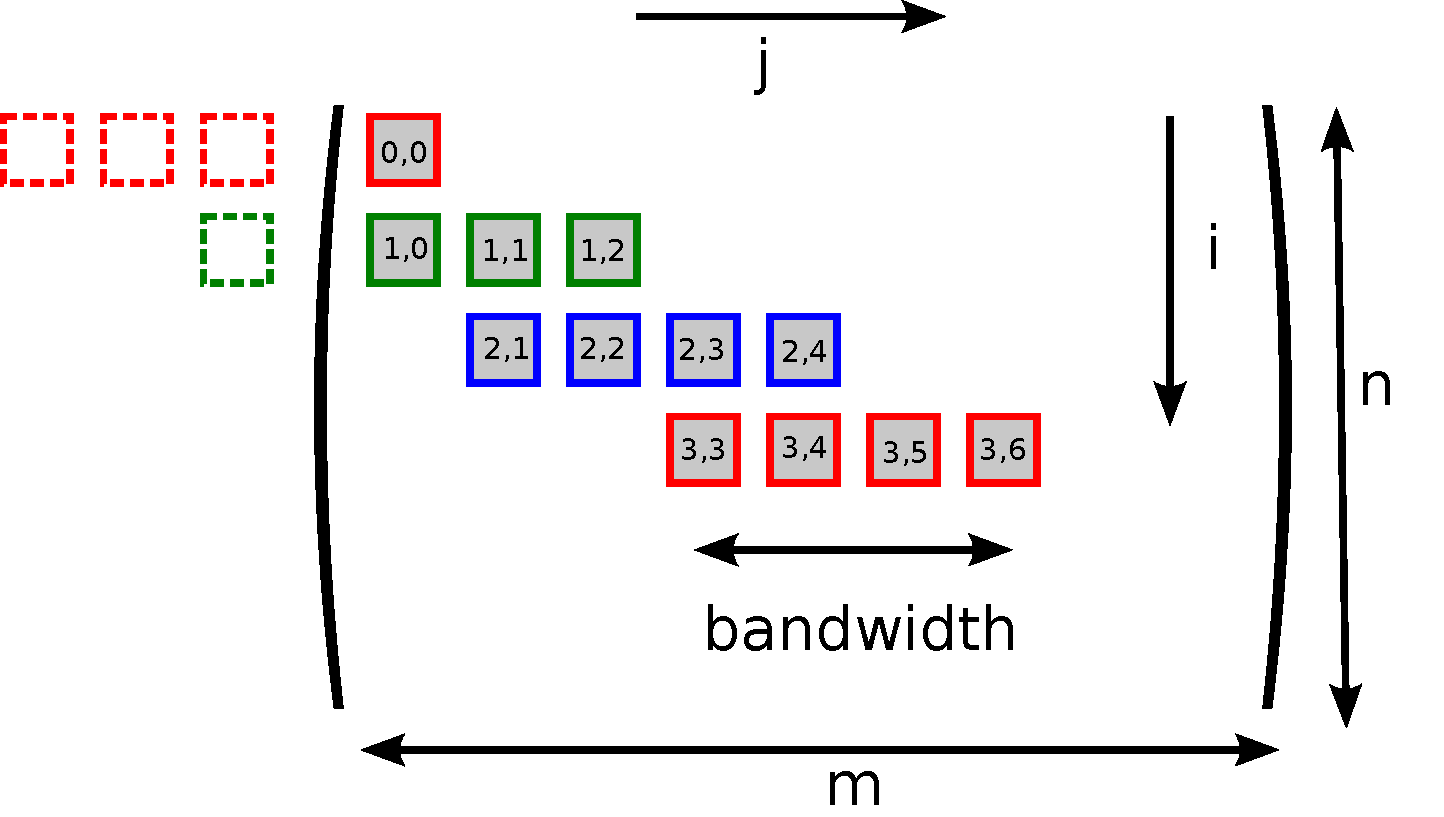
\includegraphics[width=0.6\linewidth]{bandedmatrix.pdf}
 \end{center}
 \caption{Example of a generalised banded matrix with $\alpha^{(A)}=2$, $\beta^{(A)}=1$, $\gamma^{(A)}_-=0$, $\gamma^{(A)}_+=3$ and bandwidth 4.}
 \label{fig:bandedmatrix}
\end{figure}
Without loss of generality we can assume that the greatest common divisor $G\equiv\text{gcd}(\alpha^{(A)},\beta^{(A)})$ of $\alpha^{(A)}$ and $\beta^{(A)}$ is $1$. If  $G\ne 1$, we can replace
\begin{xalignat}{3}
  \alpha^{(A)} &\mapsto \alpha^{(A)}/G, &
  \beta^{(A)} &\mapsto \beta^{(A)}/G, &
  \gamma_{\pm}^{(A)} &\mapsto \lfloor\gamma_{\pm}^{(A)}/G\rfloor
\label{eqn:gcd}
\end{xalignat}
without changing the structure of the matrix.
A special case are symmetrically banded square matrices for which $n_A=m_A$, $\alpha^{(A)}=\beta^{(A)}=1$ and $\gamma_-^{(A)}=\gamma_+^{(A)}\equiv \gamma^{(A)}$.
The number of entries per row (commonly known as the bandwidth), $n_{\text{BW}}^{(A)}$, satisfies\footnote{For $x\in \mathbb{A}$ define $\lceil x\rceil \equiv n_+$ where $n_+\in\mathbb{Z}$ is the smallest integer (positive or negative) such that $x\le n_+$. Further define $\lfloor x\rfloor = n_-$ where $n_-\in\mathbb{Z}$ is the largest integer such that $x\ge n_-$. In particular $\lceil y\rceil = \lfloor y\rfloor = y$ for $y\in\mathbb{Z}$.}
\begin{equation}
  \begin{aligned}
  \beta^{(A)}(n_{\text{BW}}-1) &\le \gamma_-^{(A)}+\gamma_+^{(A)} \\
  \Rightarrow\qquad n_{\text{BW}}^{(A)} &= 1 + \lceil\frac{\gamma_+^{(A)}+\gamma_-^{(A)}}{\beta^{(A)}}\rceil
  \end{aligned}
\end{equation}
%%%%%%%%%%%%%%%%%%%%%%%%%%%%%%%%%%%%%%%%%%%%%%%
\subsubsection{Efficient storage format}
%%%%%%%%%%%%%%%%%%%%%%%%%%%%%%%%%%%%%%%%%%%%%%%
To store these sparse matrices efficiently we can use a one-dimensional array $\overline{A}$ of length $N^{(A)}\equiv n_An_{\text{BW}}^{(A)}$ and store rows consecutively in segments of length $n_{\text{BW}}$. An index pair $(i,j)$ corresponds to position
\begin{equation}
  \nu(i,j) \equiv i\cdot n_{\text{BW}}+\left(j - j_-(i)\right)
  \qquad\text{with}\quad j_-(i) = \lceil\frac{\alpha^{(A)}i-\gamma_+^{(A)}}{\beta^{(A)}}\rceil
\end{equation}
in the array $\overline{A}$, i.e. $\overline{A}_{\nu(i,j)} = A_{ij}$, 
and this is shown in Fig. \ref{fig:linearstorage} for the matrix in Fig. \ref{fig:bandedmatrix}.
\begin{figure}
 \begin{center}
  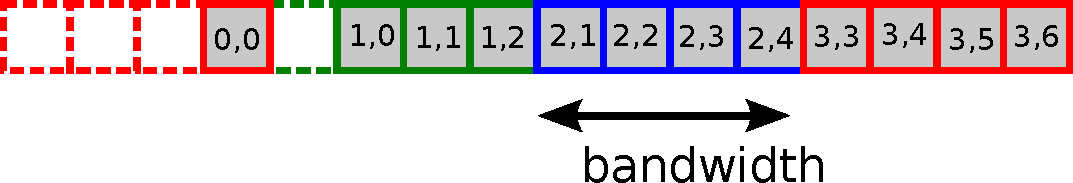
\includegraphics[width=0.5\linewidth]{linearstorage.pdf}
 \end{center}
 \caption{Linear storage for the matrix shown in Fig. \ref{fig:bandedmatrix}.}
 \label{fig:linearstorage}
\end{figure}
%%%%%%%%%%%%%%%%%%%%%%%%%%%%%%%%%%%%%%%%%%%%%%%
\subsubsection{Transpose, product and sum of generalised banded matrices}
%%%%%%%%%%%%%%%%%%%%%%%%%%%%%%%%%%%%%%%%%%%%%%%
The parameters of the transpose of a generalised banded matrix $A$ are given as
\begin{xalignat}{3}
  \alpha^{(A^T)} &= \beta^{(A)}, &
  \beta^{(A^T)} &= \alpha^{(A)}, &
  \gamma_{\pm}^{(A^T)} &= \gamma_{\mp}^{(A)}.
  \label{eqn:ParametersTranspose}
\end{xalignat}
Given a generalised banded $n_A\times m_A$ matrix $A$ and a generalised banded $n_B\times m_B$ matrix $B$ with $m_A=n_B$, the parameters of the product $AB$ are given as
\begin{xalignat}{3}
  \alpha^{(AB)} &= \alpha^{(A)}\alpha^{(B)}, &
  \beta^{(AB)} &= \beta^{(A)}\beta^{(B)}, &
  \gamma_{\pm}^{(AB)} &= \alpha^{(B)}\gamma_{\pm}^{(A)}+\beta^{(A)}\gamma_{\pm}^{(B)}
  \label{eqn:ParametersMultiply}.
\end{xalignat}
If the resulting $\alpha^{(AB)}$ and $\beta^{(AB)}$ have a greatest common divisor $G \ne 1$, divide by this as in (\ref{eqn:gcd}).

Two generalised banded $n\times m = n_A\times m_A = n_B\times m_B$ matrices $A$ and $B$ for which $\alpha^{(A)} = \alpha^{(B)}$ and
$\alpha^{(A)} = \alpha^{(B)}$ can be added with
\begin{xalignat}{3}
  \alpha^{(A+B)} &= \alpha^{(A)} = \alpha^{(B)}, &
  \beta^{(A+B)} &= \beta^{(A)} = \beta^{(B)}, &
  \gamma_{\pm}^{(A+B)} &= \max\{\gamma_{\pm}^{(A)},\gamma_{\pm}^{(B)}\}
  \label{eqn:ParametersAdd}
\end{xalignat}
%%%%%%%%%%%%%%%%%%%%%%%%%%%%%%%%%%%%%%%%%%%%%%%
\subsubsection{Operators between function spaces}
%%%%%%%%%%%%%%%%%%%%%%%%%%%%%%%%%%%%%%%%%%%%%%%
As already mentioned, in each vertical column the operator $\hat{H}_z$ is represented by a banded matrix which can be constructed from $M_p$, $M_{u,z}$ and the matrix of the derivative operator $D_z$
by using suitable multiplications and additions of banded matrices, as outlined in the previous section. 
For a grid with $n_z$ vertical layers, the parameters $\alpha^{(A)}$, $\beta^{(A)}$, $\gamma_-^{(A)}$, $\gamma_+^{(A)}$, $n^{(A)}$ and $m^{(A)}$ of the banded matrix representation $A$ of an operator mapping from function space $\Wspace_{\text{col}}$ to $\Wspace_{\text{row}}$ are given as:
\begin{equation}
  \begin{aligned}
  n^{(A)} &= n_zN_{\text{df}}^{(\text{cell})}(\Wspace_{\text{row}}) + (n_z+1)N_{\text{df}}^{(\text{facet})}(\Wspace_{\text{row}}),\\
  m^{(A)} &= n_zN_{\text{df}}^{(\text{cell})}(\Wspace_{\text{col}}) + (n_z+1)N_{\text{df}}^{(\text{facet})}(\Wspace_{\text{col}}),\\
  \alpha^{(A)} &= N_{\text{df}}^{(\text{cell})}(\Wspace_{\text{col}}) + N_{\text{df}}^{(\text{facet})}(\Wspace_{\text{col}}),\\
  \beta^{(A)} &= N_{\text{df}}^{(\text{cell})}(\Wspace_{\text{row}}) + N_{\text{df}}^{(\text{facet})}(\Wspace_{\text{row}}),\\
  \gamma_-^{(A)} &= N_{\text{df}}(\Wspace_{\text{col}})\left(N_{\text{df}}^{(\text{cell})}(\Wspace_{\text{row}}) + N_{\text{df}}^{(\text{facet})}(\Wspace_{\text{row}})\right),\\
  \gamma_+^{(A)} &= N_{\text{df}}(\Wspace_{\text{row}})\left(N_{\text{df}}^{(\text{cell})}(\Wspace_{\text{col}}) + N_{\text{df}}^{(\text{facet})}(\Wspace_{\text{col}})\right).
  \end{aligned}
\end{equation}
Here, for a given function space $\Wspace$, $N_{\text{df}}^{(\text{cell})}(\Wspace)$ is the number of degrees of freedom associated with the interior of the reference cell and $N_{\text{df}}^{(\text{facet})}(\Wspace)$ is the number of dofs associated with the bottom facet of the reference cell (for example, $N_{\text{df}}^{(\text{cell})}(\Wspace_3)=1$, $N_{\text{df}}^{(\text{facet})}(\Wspace_3)=0$ and $N_{\text{df}}^{(\text{cell})}(\Wspace_2^v)=0$, $N_{\text{df}}^{(\text{facet})}(\Wspace_2^v)=1$ at lowest order). Also we defined $N_{\text{df}}(\Wspace)\equiv N_{\text{df}}^{(\text{cell})}(\Wspace)+N_{\text{df}}^{(\text{facet})}(\Wspace)$.

%%%%%%%%%%%%%%%%%%%%%%%%%%%%%%%%%%%%%%%%%%%%%%%
\subsubsection{Algorithms}
%%%%%%%%%%%%%%%%%%%%%%%%%%%%%%%%%%%%%%%%%%%%%%%
We need to be able to carry out the following algorithms on generalised banded matrices (see appendix for explicit forms of algorithms):
\begin{itemize}
  \item Assemble banded matrix from an LMA representation of an operator (Algorithm \ref{alg:GBMMatrixAssembly})
  \item Matrix-vector products $y=Ax$ (Algorithm \ref{alg:GBMMatrixVector})
  \item Matrix-matrix products $C=AB$ (Algorithm \ref{alg:GBMMatrixMatrixProduct})
  \item Matrix-matrix sums $C=A+\omega B$ (Algorithm \ref{alg:GBMMatrixMatrixSum})
  \item Transpose matrix $B=A^T$ (Algorithm \ref{alg:GBMMatrixTranspose})
  \item Banded matrix solves $y=A^{-1}x$. This is easily achieved by using LAPACK LU- (or QR-decomposition) and solves. The LU factors can be precomputed with \texttt{dgbtrf} and stored in banded format in a preprocessing step and then \texttt{dgbtrs} can be used to carry out the forward and backward substitutions required for the solves.
  \item Sparse approximate inverse (SPAI) \cite{Grote1997}. For this prescribe a banded matrix pattern for the SPAI matrix. Calculating the entries then boils down to minimising a least squares problem in each matrix column with the LAPACK routine \texttt{dgels}.
\end{itemize}
We assume that in principle operators are available in LMA form. In each vertical column of the grid we store a three dimensional array $L^{(c)}$, such that $L^{(c)}_k$ is the local unassembled matrix with entries $\left(L^{(c)}_k\right)_{ij}$.
%%%%%%%%%%%%%%%%%%%%%%%%%%%%%%%%%%%%%%%%%%%%%%%
\subsubsection{Degree of freedom ordering and indirection maps}
%%%%%%%%%%%%%%%%%%%%%%%%%%%%%%%%%%%%%%%%%%%%%%%
For the moment we assume that the degrees of freedom in each cell are stored in firedrake-order. In each column $c$ of the grid store an indirection map $m_{\Wspace}^{(c)}$, which for each dof index $i$ in the reference cell returns the global dof index of the degrees of freedom in the lowest layer of the 3d grid. In addition, store an offset array $o_{\Wspace}$, which contains the increments which are necessary to go from one vertical layer to the next. Then the global index in an arbitrary vertical layer $k$ is given by
\begin{equation}
  i_{\text{global}} = m_{\Wspace}^{(c)}(i)+k\cdot o_{\Wspace}(i).
\end{equation}
Typically we have
\begin{equation}
  o_{\Wspace}(i)=N_{\text{df}}^{(\text{cell})}(\Wspace)+N_{\text{df}}^{(\text{facet})}(\Wspace)\qquad\text{for all $i$}.
\end{equation}
%%%%%%%%%%%%%
\newcommand{\Ndfrow}{N_{\text{df}}(\Wspace_{\text{row}})}
\newcommand{\Ndfcellrow}{N_{\text{df}}^{(\text{cell})}(\Wspace_{\text{row}})}
\newcommand{\Ndffacetrow}{N_{\text{df}}^{(\text{facet})}(\Wspace_{\text{row}})}
\newcommand{\Ndfcol}{N_{\text{df}}(\Wspace_{\text{row}})}
\newcommand{\Ndfcellcol}{N_{\text{df}}^{(\text{cell})}(\Wspace_{\text{col}})}
\newcommand{\Ndffacetcol}{N_{\text{df}}^{(\text{facet})}(\Wspace_{\text{col}})}
%%%%%%%%%%%%%%%%%%%%%%%%%%%%%%%%%%%%%%%%%%%%%%%
\subsubsection{Construction of banded diagonal matrix $\hat{H}_z$}
%%%%%%%%%%%%%%%%%%%%%%%%%%%%%%%%%%%%%%%%%%%%%%%
To construct the banded diagonal matrix in each cell we can proceed as follows:
\begin{enumerate}
  \item Assemble $M_p$, $M_{u,z}$, $M_{u,h}$, $D_z$ and $D_h$ into their local matrix (LMA) representation $L[M_p]$ etc.
  \item Assemble the local matrix representations into banded matrices using algorithm \ref{alg:GBMMatrixAssembly}, transpose the banded matrix for $D_z$ using algorithm \ref{alg:GBMMatrixTranspose}
  \item Calculate $M_{u,h,\text{inv}}$, e.g. using (\ref{eqn:horizontalMassLumping})
  \item Calculate the sparse approximate inverse $M_{u,z,\text{inv}}$ by solving a least squares problem for each matrix column as described in \cite{Grote1997}.
  \item Calculate $\Delta_h$ using algorithm \ref{alg:GBMDeltahAssembly}
  \item Build $\hat{H}_z = M_p+\omega_c^2\Delta_h+\omega_c^2/(1+\omega_N^2) D_z M_{u,z,\text{inv}}D_z^T$ using algorithms \ref{alg:GBMMatrixMatrixProduct} and \ref{alg:GBMMatrixMatrixSum}
  \item LU-factorise $\hat{H}_z$ using LAPACK.
\end{enumerate}

%%%%%%%%%%%%%%%%%%%%%%%%%%%%%%%%%%%%%%%%%%%%%%%
\appendix
\section{Algorithms}
%%%%%%%%%%%%%%%%%%%%%%%%%%%%%%%%%%%%%%%%%%%%%%%
The explicit form of the algorithms described above is given here.
\begin{algorithm}[H]
 \caption{Generalised banded matrix assembly from local matrix (LMA) representation $L[A]_k$}
 \label{alg:GBMMatrixAssembly}
 \begin{algorithmic}[1]
   \STATE{$\overline{A}\mapsto 0$}
   \FOR{$k=0$ \TO $n_z-1$}
     \FOR{$I=0,\Ndfrow-1$}
\STATE{$i=k\cdot o_{\text{row}}(I)+m^{(c)}_{\text{row}}(I)$}
         \STATE{$j_-=\lceil(\alpha^{(A)}i-\gamma_+^{(A)})/\beta^{(A)}\rceil$}
       \FOR{$J=0,\Ndfcol-1$}
                  \STATE{$j=k\cdot o_{\text{col}}(J)+m^{(c)}_{\text{col}}(J)$} 
         \STATE{$\overline{A}_{BW^{(A)}i+(j-j_m)}\mapsto\overline{A}_{BW^{(A)}i+(j-j_-)}+\left(L[A]_k\right)_{I,J}$}
       \ENDFOR
     \ENDFOR
   \ENDFOR
 \end{algorithmic}
\end{algorithm}

\begin{algorithm}[H]
 \caption{Generalised banded \texttt{axpy} matrix-vector multiplication $y\mapsto y+Ax$}
 \label{alg:GBMMatrixVector}
 \begin{algorithmic}[1]
   \FOR{$i=0$ \TO $n_A-1$}
     \STATE{$s\mapsto 0$}
     \STATE{$j_- = \lceil (\alpha^{(A)}i-\gamma_+^{(A)})/\beta^{(A)}\rceil$}
     \STATE{$j_+ = \lfloor (\alpha^{(A)}i+\gamma_-^{(A)})/\beta^{(A)}\rfloor$}
     \FOR{$j=\max\{0,j_-\}$ \TO $\min\{m_A-1,j_+\}$}
       \STATE{$s \mapsto s + \overline{A}_{n_{\text{BW}}^{(A)}i+(j-j_-)} x_j$}
     \ENDFOR
     \STATE{$y_i\mapsto y_i+s$}
   \ENDFOR
 \end{algorithmic}
\end{algorithm}

\begin{algorithm}[H]
 \caption{Generalised banded matrix-matrix multiplication $C=AB$}
 \label{alg:GBMMatrixMatrixProduct}
 \begin{algorithmic}[1]
   \STATE{$\overline{C}\mapsto 0$}
   \FOR{$i=0$ \TO $n_A-1$}
     \STATE{$j_- = \lceil (\alpha^{(C)}i-\gamma_+^{(C)})/\beta^{(C)}\rceil$}
     \STATE{$j_+ = \lfloor (\alpha^{(C)}i+\gamma_-^{(C)})/\beta^{(C)}\rfloor$}
     \STATE{$k_- = \lceil (\alpha^{(A)}i-\gamma_+^{(A)})/\beta^{(A)}\rceil$}
     \STATE{$k_+ = \lfloor (\alpha^{(A)}i+\gamma_-^{(A)})/\beta^{(A)}\rfloor$}
     \FOR{$j=\max\{0,j_-\}$ \TO $\min\{m_B-1,j_+\}$}
       \STATE{$s\mapsto 0$}
       \FOR{$k=\max\{0,k_-\}$ \TO $\min\{m_A-1,k_+\}$}
         \IF{$\lceil(\alpha^{(B)}k-\gamma_-^{(B)})/\beta^{(B)}\rceil\le j \le \lfloor(\alpha^{(B)}k+\gamma_+^{(B)})/\beta^{(B)}\rfloor$}
           \STATE{$j'_- = \lceil (\alpha^{(B)}k-\gamma_+^{(B)})/\beta^{(B)}\rceil$}
           \STATE{$s = s + \overline{A}_{n_{\text{BW}}^{(A)}i+(k-k_-)}\overline{B}_{n_{\text{BW}}^{(B)}k+(j-j'_-)}$}
         \ENDIF
       \ENDFOR
       \STATE{$\overline{C}_{n_{\text{BW}}^{(C)}i+(j-j_-)}\mapsto  s$}
     \ENDFOR
   \ENDFOR
 \end{algorithmic}
\end{algorithm}

\begin{algorithm}[H]
 \caption{Generalised banded matrix-matrix addition $C=A+\omega B$}
 \label{alg:GBMMatrixMatrixSum}
 \begin{algorithmic}[1]
   \STATE{$\overline{C}\mapsto 0$}
   \FOR{$i=0$ \TO $n_A-1$}
     \STATE{$j^{(A)}_- = \lceil (\alpha^{(A)}i-\gamma_+^{(A)})/\beta^{(A)}\rceil$}
     \STATE{$j^{(A)}_+ = \lfloor (\alpha^{(A)}i+\gamma_-^{(A)})/\beta^{(A)}\rfloor$}
     \STATE{$j^{(B)}_- = \lceil (\alpha^{(B)}i-\gamma_+^{(B)})/\beta^{(B)}\rceil$}
     \STATE{$j^{(B)}_+ = \lfloor (\alpha^{(B)}i+\gamma_-^{(B)})/\beta^{(B)}\rfloor$}
     \STATE{$j^{(C)}_- = \lceil (\alpha^{(C)}i-\gamma_+^{(C)})/\beta^{(C)}\rceil$}
     \STATE{$j^{(C)}_+ = \lfloor (\alpha^{(C)}i+\gamma_-^{(C)})/\beta^{(C)}\rfloor$}
     \FOR{$j=\max\{0,j^{(A)}_-\}$ \TO $\min\{m_A-1,j^{(A)}_+\}$}
       \STATE{$\overline{C}_{n_{\text{BW}}^{(C)}i+(j-j^{(C)}_-)}=\overline{C}_{n_{\text{BW}}^{(C)}i+(j-j^{(C)}_-)}+\overline{A}_{n_{\text{BW}}^{(A)}i+(j-j^{(A)}_-)}$}
     \ENDFOR
     \FOR{$j=\max\{0,j^{(B)}_-\}$ \TO $\min\{m_A-1,j^{(B)}_+\}$}
       \STATE{$\overline{C}_{n_{\text{BW}}^{(C)}i+(j-j^{(C)}_-)}=\overline{C}_{n_{\text{BW}}^{(C)}i+(j-j^{(C)}_-)}+\omega\overline{B}_{n_{\text{BW}}^{(B)}i+(j-j^{(B)}_-)}$}
     \ENDFOR
   \ENDFOR
 \end{algorithmic}
\end{algorithm}

\begin{algorithm}[H]
 \caption{Generalised banded matrix transpose $B=A^T$}
 \label{alg:GBMMatrixTranspose}
 \begin{algorithmic}[1]
   \FOR{$i=0$ \TO $n_A-1$}
     \STATE{$j_- = \lceil (\alpha^{(A)}i-\gamma_+^{(A)})/\beta^{(A)}\rceil$}
     \STATE{$j_+ = \lfloor (\alpha^{(A)}i+\gamma_-^{(A)})/\beta^{(A)}\rfloor$}
     \FOR{$j=\max\{0,j_-\}$ \TO $\min\{m_B-1,j_+\}$}
       \STATE{$i_- = \lceil (\beta^{(A)}j-\gamma_-^{(A)})/\alpha^{(A)}\rceil = \lceil (\alpha^{(B)}j-\gamma_+^{(B)})/\beta^{(B)}\rceil$}
       \STATE{$\overline{B}_{n_{\text{BW}}^{(B)}j+(i-i_-)}\mapsto \overline{A}_{n_{\text{BW}}^{(A)}i+(j-j_-)}$}
     \ENDFOR
   \ENDFOR
 \end{algorithmic}
\end{algorithm}

\newcommand{\ndfWthree}{N_{\text{df}}(\Wspace_3)}
\newcommand{\ndfWtwov}{N_{\text{df}}(\Wspace_2^v)}
\begin{algorithm}
 \caption{Assembly of banded matrix for $\Delta_h=\text{diag}_h\left(D_hM_{u,h,\text{inv}}D_h^T\right)$ from the local matrix (LMA) representations $L[D_h]$ and $L[M_{u,h,\text{inv}}]$}
 \label{alg:GBMDeltahAssembly}
 \begin{algorithmic}[1]
   \STATE{$\overline{\Delta}_h\mapsto 0$}
   \FOR{$k=0$ \TO $n_z-1$}
     \FOR{$I=0,\ndfWthree-1$}
\STATE{$i=k\cdot o_{\Wspace_3}(I)+m^{(c)}_{\Wspace_3}(I)$}
       \FOR{$J=0,\ndfWtwov-1$}
                  \STATE{$j=k\cdot o_{\Wspace_2^v}(J)+m^{(c)}_{\Wspace_2^v}(J)$} 
         \STATE{$s=0$}
     \FOR{$L=0,\ndfWtwov-1$}
       \FOR{$M=0,\ndfWtwov-1$}
        \STATE{$s\mapsto s+\left(L[D_h]_k\right)_{IL}\cdot\left(L[M_{u,h,\text{inv}}]\right)_{LM}\cdot\left(L[D_h]_k\right)_{JM}$}
       \ENDFOR
     \ENDFOR

\STATE{$j_-=\lceil(\alpha^{(A)}i-\gamma_+^{(A)})/\beta^{(A)}\rceil$}
         \STATE{$\left(\overline{\Delta}_h\right)_{BW^{(A)}i+(j-j_-)}\mapsto\left(\overline{\Delta}_h\right)_{BW^{(A)}i+(j-j_-)}+s$}
       \ENDFOR
     \ENDFOR
   \ENDFOR
 \end{algorithmic}
\end{algorithm}
%%%%%%%%%%%%%%%%%%%%%%%%%%%%%%%%%%%%%%%%%%%%%%%
%%%%%%%%%%%%%%%%%%%%%%%%%%%%%%%%%%%%%%%%%%%%%%%

\bibliographystyle{plain}
\bibliography{GravityWaves}
\end{document}
